\documentclass{article}
\usepackage[utf8]{vietnam}
\usepackage{graphicx}
\usepackage{amsmath}
\usepackage{amssymb}
\usepackage{hyperref}
\usepackage{caption}
\usepackage{subcaption}

\title{Geometric Transformations\\ \Large Report Lab Week 5-6 Part1}
\author{Ngọc Thuận - IPSAL LAB}
\date{January 2023}

\begin{document}

\maketitle
\begin{abstract}
Trong những bài trước, chúng ta đã nghiên cứu về ảnh kĩ thuật số (digital images) nhưng là về những khía cạnh bên trong của bức ảnh, cấu tạo ra sao, thể hiện như nào\ldots Chúng ta đã biết tương đối các phương pháp cơ bản và phổ thông trong xử lí ảnh cổ điển. Trong bài này, cũng sẽ là phần cuối của xử lí ảnh cơ bản, ta sẽ nghiên cứu về một mảng cũng rất thú vị của xử lí ảnh, đó là Biến đổi hình học của ảnh (Geometric Transformations). Bài này sẽ cung cấp một số kiến thức cơ bản về phép biến đổi hình học, trong đó có cách xây dựng, một số phép biến đổi thông dụng và một số ứng dụng của phép biến đổi hình học.  
\end{abstract}
\tableofcontents
\newpage
\section{Introduction}
"Kìa trong gió là trái tim biết yêu, là tình yêu vẫy gọi chút màu nắng. Bức tranh anh để nơi tim mình, một chút thương nhớ, chẳng thể nào phôi pha\ldots":\\
\begin{figure}[ht!]
    \centering
    \begin{subfigure}[b]{0.7\linewidth}             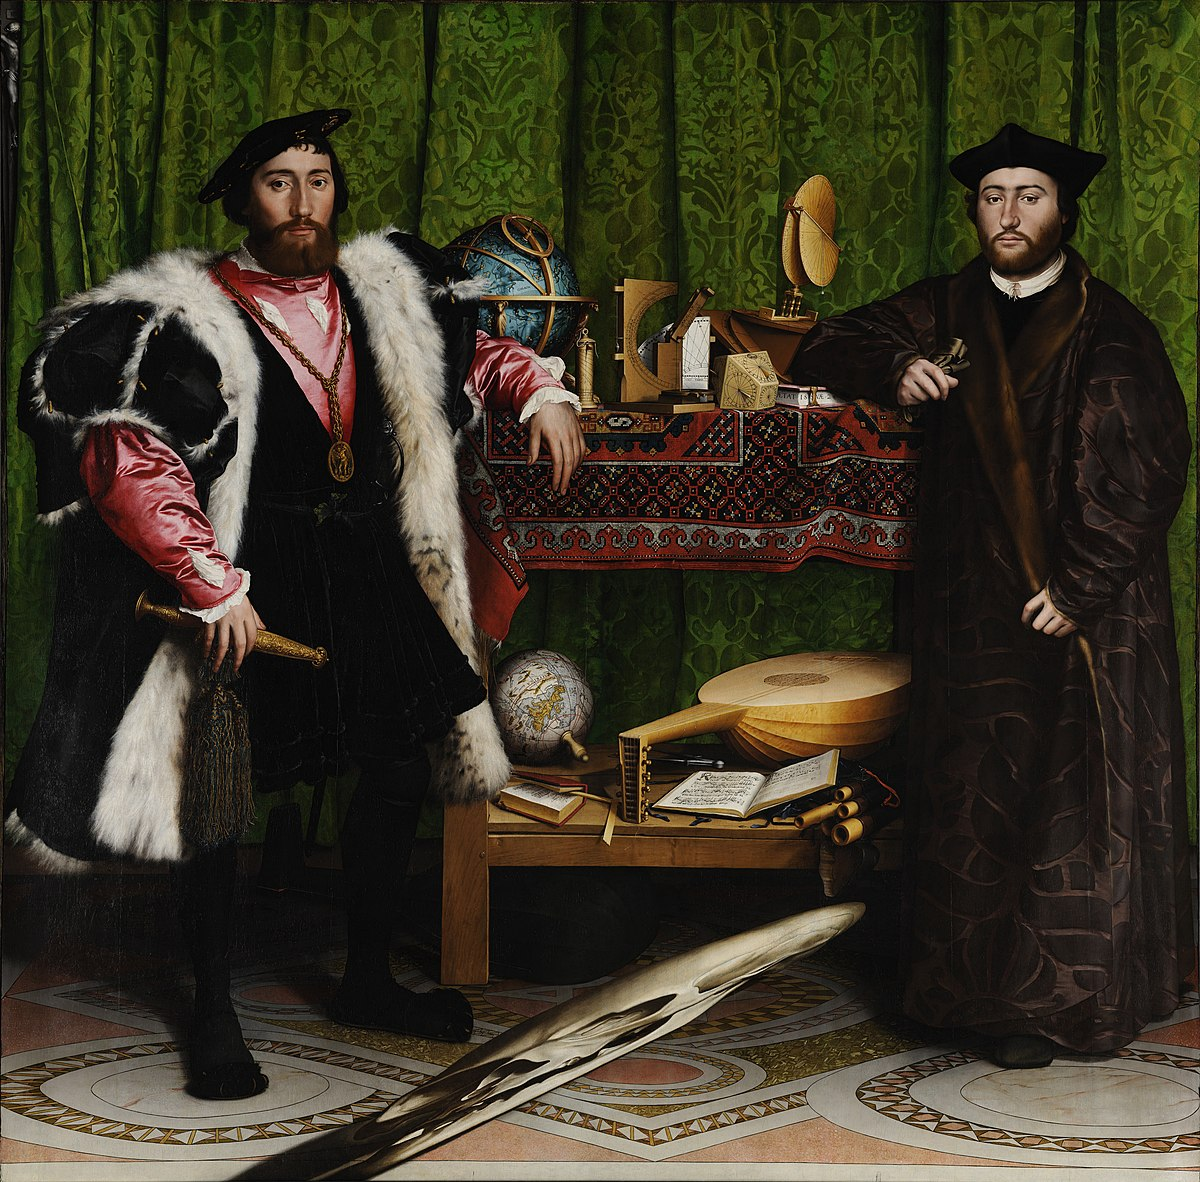
\includegraphics[width=\linewidth]{holbein.jpg}
    \caption{Holbein, “The Ambassadors”}
    \end{subfigure}
    
    \begin{subfigure}[b]{0.7\linewidth}           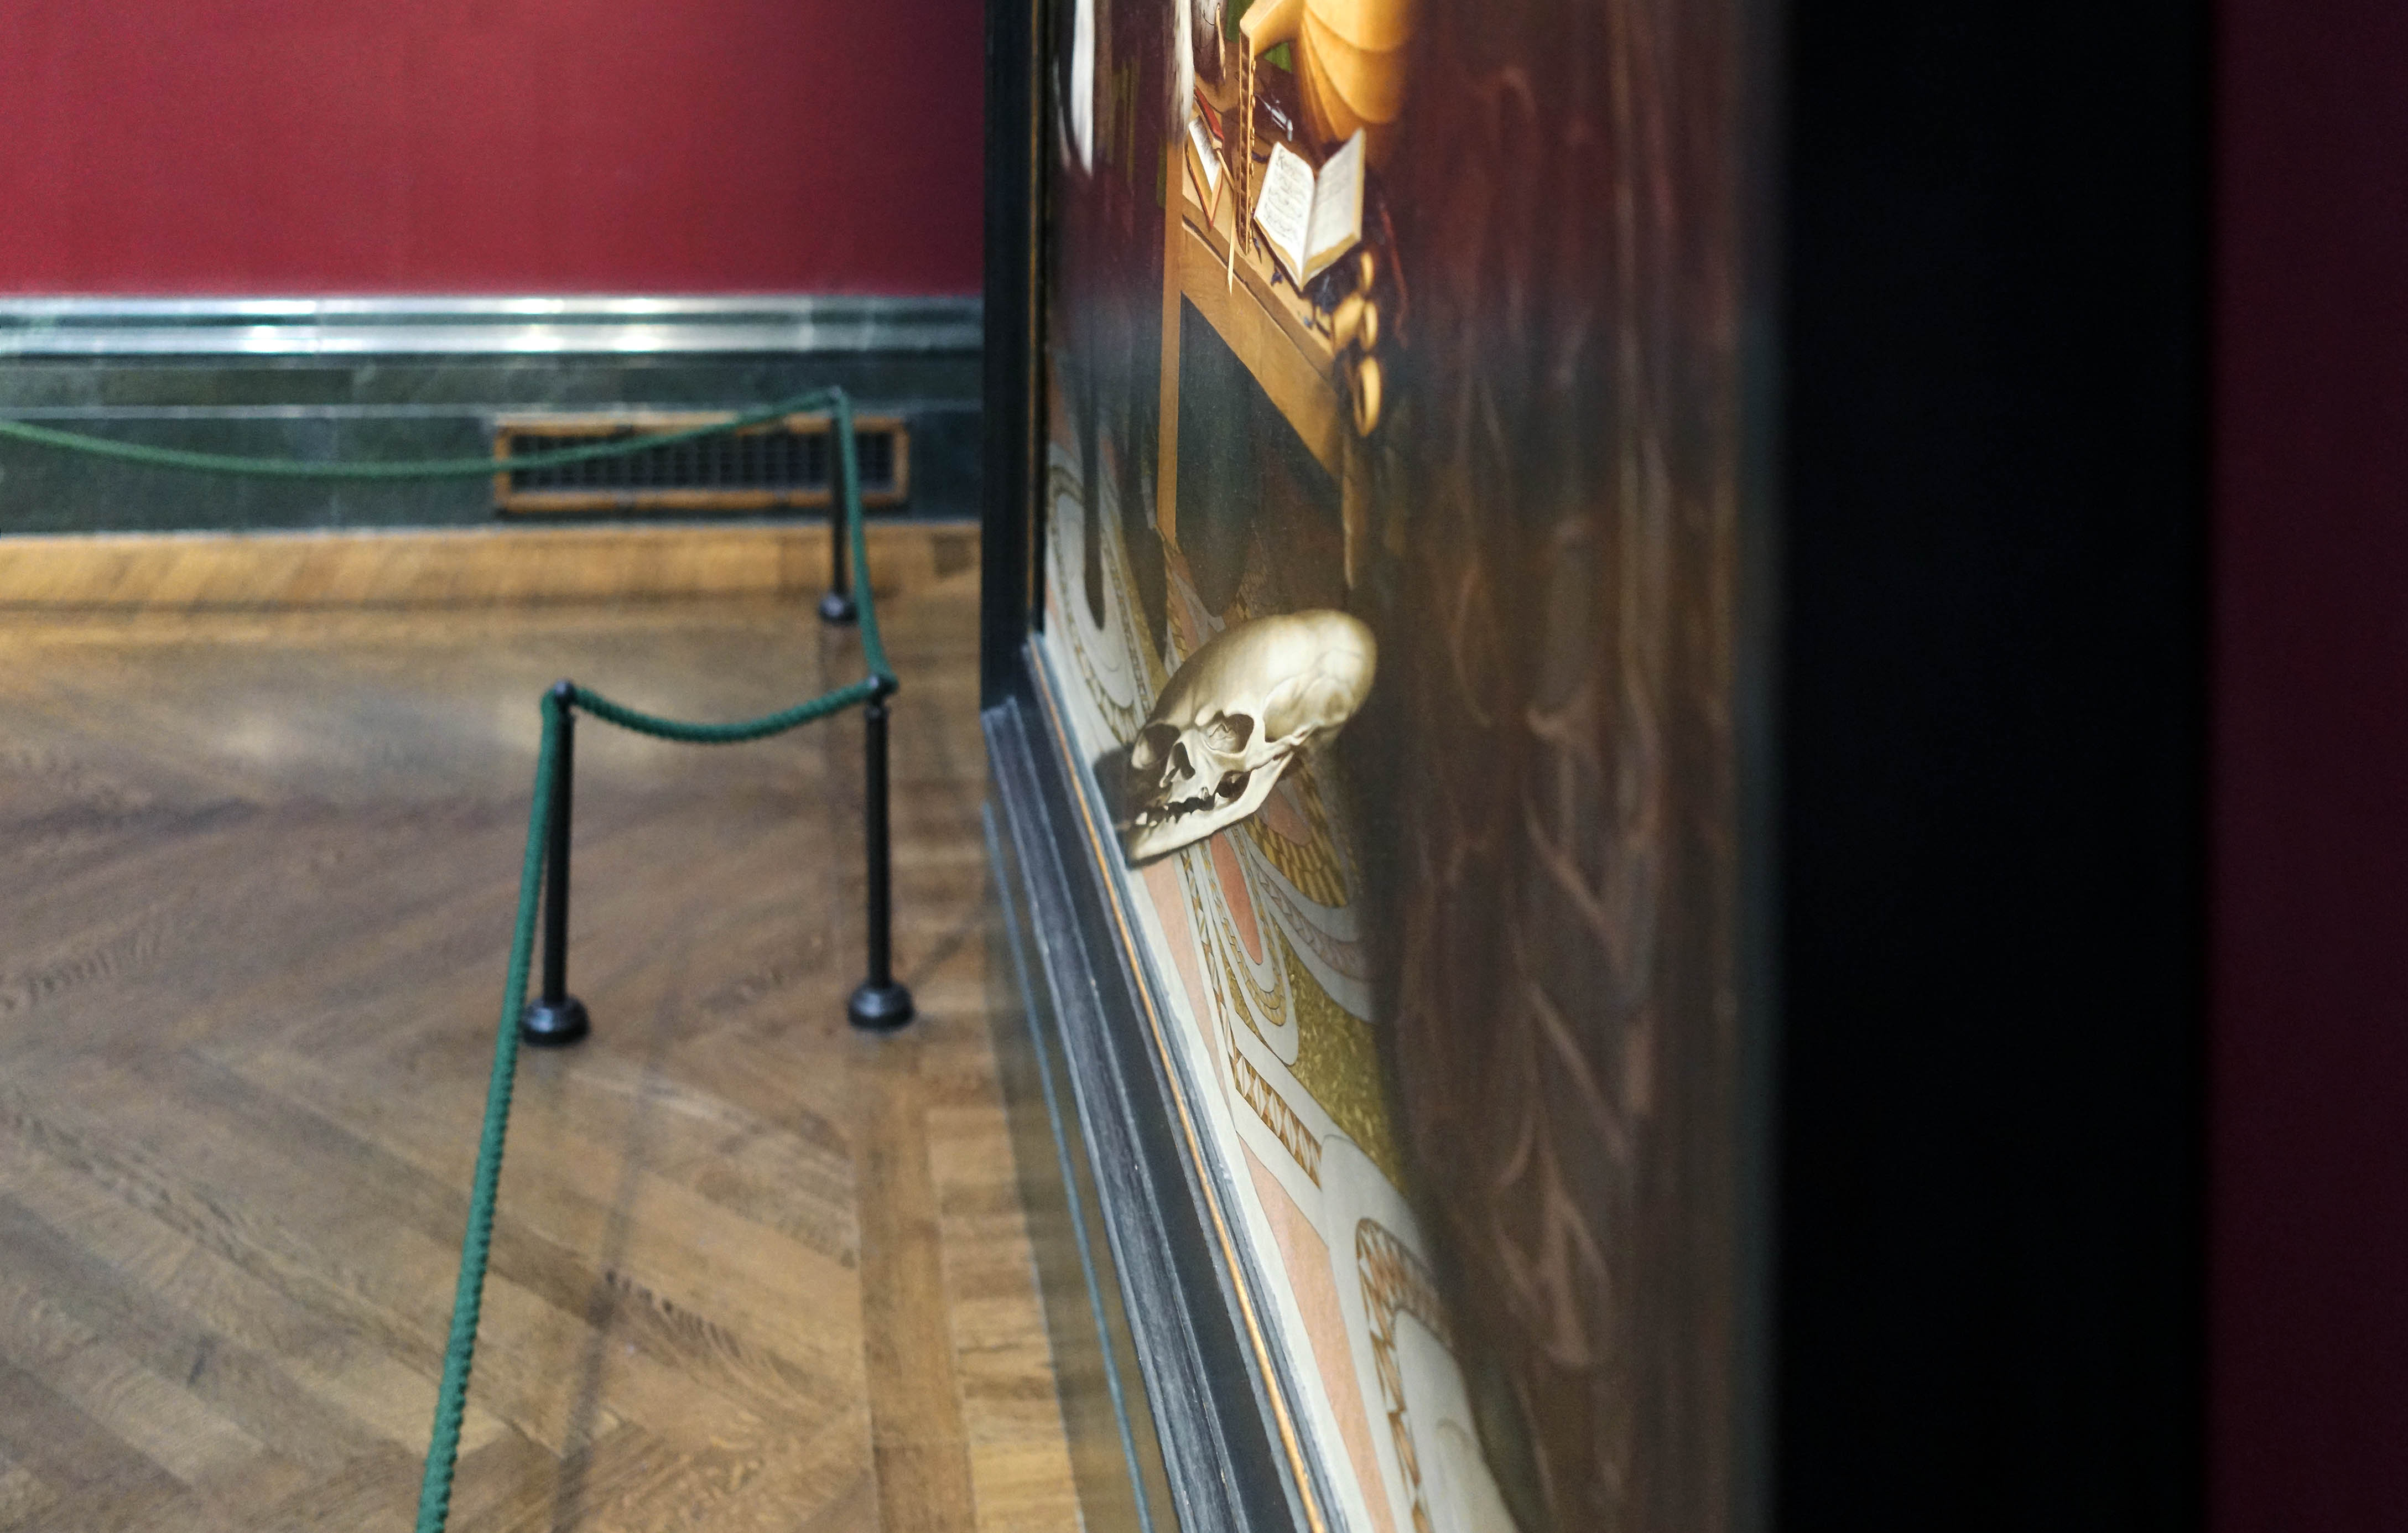
\includegraphics[width=\linewidth]{HolbeinSkullCorrected.jpg}
    \caption{Another view}
    \end{subfigure}
    
    \caption{A weird painting!!! 
    }\href{https://en.wikipedia.org/wiki/The_Ambassadors_%28Holbein%29}{The Ambassadors}
    \label{fig1}
\end{figure}

Hình \ref{fig1} là một bức tranh khá thú vị, bạn thấy gì ở bức tranh đầu (Hình a)?. Lẽ ra để cho khớp với lời dẫn trên, tôi phải dùng hình ảnh khác, phải chim hoa bướm lượn, phải ngọt ngào chìm đắm, phải nồng nàn mãnh liệt \ldots thay vì hai ông thi nhau tự sướng!\\
Tuy nhiên bài này không phải nghiên cứu về tranh, bức tranh này thật sự đặc biệt nếu bạn để ý. Bên cạnh những nét vẽ tinh xảo, chi tiết khắc họa hai ông quý tộc kia thì còn một chi tiết nữa rõ nổi bật, và có lẽ chính nó làm bức họa trở nên đẹp và khác biệt hơn! Hình (b) là khi ta nhìn chéo bức tranh. Bạn thấy rồi chứ? Điều kì diệu trong bức tranh ấy? Đó cũng là thứ ta sẽ bàn luận trong phạm vi bài này! Ta có quyền đặt câu hỏi, có cách nào để công thức hóa góc nhìn con người không? Hay ý là có cách nào để từ bức ảnh thu được từ góc độ này, qua một vài phép biến đổi ta có thể thu gián tiếp được bức ảnh tương tự khi thu ở góc độ khác? Câu trả lời hiển nhiên là có (ta gọi đây là các \textit{phép biến đổi hình học}) và trước khi bắt đầu, chúng ta hãy cùng xem một vài bức ảnh sau, đó là kết quả sau khi trả lời được câu hỏi trên, và cũng là những ứng dụng cơ bản nhất mà tôi có thể giới thiệu trong phạm vi bài này!\\
\begin{figure}[ht!]
    \centering
    \begin{subfigure}[b]{0.6\linewidth}             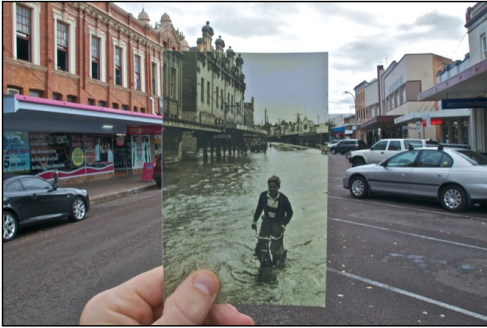
\includegraphics[width=\linewidth]{fig1.png}
    \caption{Image registration}
    \end{subfigure}
    
    \begin{subfigure}[b]{0.6\linewidth}           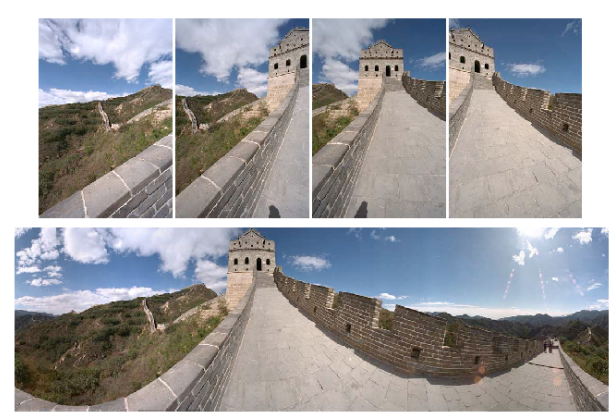
\includegraphics[width=\linewidth]{fig2.png}
    \caption{Image stitching}
    \end{subfigure}

    \caption{Some exciting applications of geometric transformations}
    \label{fig2}
\end{figure}
\section{Cơ sở toán học}
Nhắc lại một chút về kiến thức đại số tuyến tính. 
\subsection{Không gian vector}
Tôi sẽ không đề cập đến định nghĩa của không gian \textit{vector}, vì định nghĩa khá dài dòng, có thể tóm tắt là một không gian \textit{vector} \textbf{E} trên trường K là tập hợp phải thỏa mãn 8 tiên đề cơ bản. \\
Gần giũ nhất với chúng ta, ta có tập hợp các \textit{vector} hình học, có gốc là gốc tọa độ. Xin nhắc lại là phải có gốc tọa độ, vì tiên đề yêu cầu không gian \textit{vector} phải có \textit{vector} \textbf{0}.
\subsubsection*{Cơ sở và tọa độ}
\label{n1}
Có nhiều cách để định nghĩa cơ sở, nhưng để ngắn gọn tôi sẽ sử dụng định lí sau cho cả cơ sở và tọa độ:\\
\fbox{
\begin{minipage}{\linewidth}
\textbf{Định lí:} Tập $S = \left\{ \textbf{x}_{i} \right\}$ là một cơ sở của \textbf{E} khi và chỉ khi mọi \textit{vector} của \textbf{E} đều có thể viết dưới dạng $\textbf{x} = \sum_{i} {a_i}{\textbf{x}_i}$ với các hệ số $a_i$ xác định một cách duy nhất theo $\textbf{x}$ 
\end{minipage}
}
\phantom{a}\\
Định lí này ngoài cho ta khái niệm về cơ sở, còn cho ta khái niệm về tọa độ. Với một cơ sở cho trước, mỗi \textit{vector} xác định duy nhất một bộ số, bộ số đó chính là tọa độ của chúng.\\
Điều này dẫn đến một điều dễ hiểu, một không gian \textit{vector} có nhiều cơ sở, và một \textit{vector} có vô vàn tọa độ, phụ thuộc vào cơ sở được chọn.\\
Trong không gian \textit{vector} hình học trên không gian $d$ chiều, có gốc là gốc tọa độ có bộ cơ sở chuẩn tắc ${\textbf{e}_i} = (x_1,x_2,\ldots, x_d)$:
$$
x_k = 
\begin{cases}
1, \text{ if } k = i\\
0, \text{ otherwise }
\end{cases}
$$
Qua đây ta thấy, tọa độ trực chuẩn của một \textit{vector} trong không gian \textit{vector} trên, chính là tọa độ điểm cuối \textit{vector} trong không gian \textit{Descartes}.

\underline{Hệ quả}:
Ta có một số hệ quả quan trọng sau
\begin{enumerate}
    \item S là hệ sinh cực tiểu của \textbf{E}.
    \item S là hệ độc lập tuyến tính cực đại của \textbf{E}.
    \item $\dim \textbf{E} = n_S$, $n_S$: số \textit{vectors} của cơ sở.
    \item Ma trận tạo bởi các \textit{vector} của cơ sở luôn khả nghịch.
\end{enumerate}
\subsubsection*{Công thức đổi tọa độ}
Câu hỏi đặt ra là: \textit{Liệu có mối quan hệ giữa tọa độ của một vector đối với hai cơ sở khác nhau?}. Câu trả lời là có! Ta sẽ cùng thiết lập nó:\\
Giả sử cho không gian \textit{vector} \textit{E}, \textit{vector} $\textbf{x} \in \textbf{E}$ và hai bộ cơ sở $A = \{\textbf{a}_i\}, B = \{\textbf{b}_i\}$. Kí hiệu $[x]_A = [x_1^a; x_2^a; \ldots ;x_d^a]$ là tọa độ của \textit{vector} $\textbf{x}$ đối với cơ sở $A$, tương tự với $B$ $[x]_B = [x_1^b; x_2^b; \ldots; x_d^b]$.\\ \\
\underline{Lưu ý}: Phân biệt dấu `,' và dấu `;'. `,' ta sẽ dùng kí hiệu cho các \textit{vector} hàng, và `;' ta sẽ dùng kí hiệu cho các \textit{vector} cột.\\ \\%
Theo định nghĩa ta có: $$\textbf{x} = \sum_{i}{a_i}{\textbf{x}_i^a} = \sum_{i}{b_I}{\textbf{x}_i^b}$$
Suy ra, $$[\textbf{a}_1; \textbf{a}_2; \ldots; \textbf{a}_d][x]_{A} = [\textbf{b}_1; \textbf{b}_2; \ldots; \textbf{b}_d][x]_{B}$$
$$\iff [x]_{B} = [\textbf{b}_1; \textbf{b}_2; \ldots; \textbf{b}_d]^{-1}[\textbf{a}_1; \textbf{a}_2; \ldots; \textbf{a}_d][x]_{A}$$
Đặt $[A]_{B} = [\textbf{b}_1; \textbf{b}_2; \ldots; \textbf{b}_d]^{-1}[\textbf{a}_1; \textbf{a}_2; \ldots; \textbf{a}_d]$(*), ta được công thức chuyển tọa độ:
$$\fbox{$[x]_{B} = [A]_{B}[x]_{A} = [B]_{A}^{-1}[x]_A$}$$
Có lẽ (*) vẫn còn khá mơ hồ, ta sẽ tiếp tục biến đổi (*):
$$(*) \iff [A]_{B} =  \left[[\textbf{b}_1; \textbf{b}_2; \ldots; \textbf{b}_d]^{-1} \textbf{a}_1; [\textbf{b}_1; \textbf{b}_2; \ldots; \textbf{b}_d]^{-1} \textbf{a}_2; \ldots; [\textbf{b}_1; \textbf{b}_2; \ldots; \textbf{b}_d]^{-1} \textbf{a}_d \right]$$
$ \phantom{(*)} \iff [A]_{B} = [[\textbf{a}_1]_{B}; [\textbf{a}_2]_{B}; \ldots; [\textbf{a}_d]_{B}]$\\ \\
Thì ra, $A_B$ là ma trận hợp tọa độ đối với cơ sở $B$ của các \textit{vector} trong cơ sở $A$.

%\subsection{Ánh xạ tuyến tính}
%\fbox{
%\begin{minipage}{\linewidth}
%Cho $E$ và $F$ là hai không gian \textit{vector} trên trường $K$. Một ánh xạ %$\phi$:E $\rightarrow$ F được gọi là một ánh xạ tuyến tính nếu:
%\begin{enumerate}
%    \item $\phi(x+y) = \phi(x)+\phi(y)$
%    \item $\phi(\alpha x) = \alpha \phi(x)$
%\end{enumerate}
%    với mọi $x, y \in E$ và $\alpha \in K$.
%\end{minipage}
%}
%\\

%%Trong thực tế, ta thường xét $E, F$ là các không gian thực đa chiều, và trường $K$ là trường số thực. Hơn nữa ta có cách phát biểu khác dễ tiếp cận hơn cho ánh xạ tuyến tính như sau:
%$$y = Ax$$ với $y \in \mathbb{R}^{m}$, $x \in \mathbb{R}^{n}$ và $A \in \mathbb{R}^{m \times n}$. Trong trường hợp $m=n$, ánh xạ tuyến tính còn được gọi là \textit{toán tử tuyến tính}.

\subsection{Không gian Affine}
\label{n2}
\subsubsection*{Định nghĩa}
\fbox{
\begin{minipage}{\linewidth}
Cho một tập \textbf{A} $\neq \varnothing$ (phần tử của \textbf{A} gọi là điểm), một K-không gian \textit{vector} \textbf{V} và một ánh xạ
$$\Phi = \textbf{A} \times \textbf{A} \rightarrow \textbf{V} $$
$$(A,B) \mapsto \overrightarrow{AB}$$
sao cho:
\begin{enumerate}
    \item Giữ cố định A thì ánh xạ B $\in \textbf{A} \mapsto \overrightarrow{AB} \in \textbf{V}$ là một song ánh
    \item Với A, B, C thuộc \textbf{A} có $\overrightarrow{AB} + \overrightarrow{BC} = \overrightarrow{AC}$
\end{enumerate}
Bộ ba $(\textbf{A}, \textbf{V}, \Phi)$ hay tập \textbf{A} gọi là một \textit{K - không gian affine} liên kết với không gian \textit{vector} \textbf{V} bởi ánh xạ $\Phi$
\end{minipage}
}\\

Trong toán học, không gian \textit{affine} là một cấu trúc hình học tổng quát tính chất của các đường thẳng song song trong không gian \textit{Euclide}. Trong không gian \textit{affine}, không định nghĩa một điểm đặc biệt nào làm gốc. Do đó, không \textit{vector} nào có gốc cố định và không \textit{vector} nào có thể liên kết được duy nhất với một điểm. Thay vào đó, các nhà toán học định nghĩa các \textit{vector} nối giữa hai điểm trong không gian \textit{affine}. Vì vậy, khi trừ hai điểm của không gian sẽ cho một \textit{vector}, nhưng sẽ không có nghĩa khi cộng hai điểm trong không gian \textit{affine}. Tương tự, có thể cộng một \textit{vector} với một điểm trong không gian, kết quả thu được là một điểm mới tịnh tiến dọc theo \textit{vector} từ điểm bắt đầu của \textit{vector}. \\Tham khảo thêm \href{https://vi.wikipedia.org/wiki/Kh%C3%B4ng_gian_afin}{Không gian affine}

\subsubsection*{Tọa độ affine trong A}
Hệ thống $S:(O, \textbf{e}_1, \textbf{e}_2,\ldots, \textbf{e}_n)$ gồm O $\in \textbf{A}$, $(\textbf{e}_1, \textbf{e}_2, \ldots, \textbf{e}_n)$ là cơ sở của \textbf{V} gọi là \textit{hệ tọa độ affine} trong \textbf{A}.\\
$M \in \textbf{A}$ thì $\overrightarrow{OM} = \sum_{i=1}^{n}$ thì ta nói M có tọa độ $[x_1;x_2;\ldots;x_n]$ trong hệ tọa độ đó. Ta kí hiệu tương tự phần trên.\\
Xét hệ tọa độ $S':(O', \textbf{e}_1', \textbf{e}_2', \textbf{e}_3',\ldots, \textbf{e}_4')$, $\overrightarrow{OO'} = \sum_{i=1}^{n}b_i \textbf{e}_i = [O']_S= \textbf{b}$, $C = [S']_{S}$. Khi đó ta có công thức:
\begin{equation}
    [x]_{S} = C[x']_{S'}+\textbf{b}
    \label{eq1}
\end{equation}
Công thức (\ref{eq1}) được gọi là \textit{Công thức đổi tọa độ affine}. 
\section{Geometric Transformations}
Sau đây ta sẽ đi vào phần chính của bài, những cơ sở toán trên là gốc rễ cho những kết quả này. Trong phần này tôi sẽ giới thiệu sơ qua về khái niệm \textit{phép biến đổi hình học} và hai phép biến đổi phổ biến: \textit{affine} và \textit{projective transformations}.
\subsection{Định nghĩa}
Ta có thể định nghĩa đơn giản, \textit{Phép biến đổi hình học}, là thông qua một toán tử $T$, ta biến không gian này thành không gian khác, giữa các điểm ta có:
$$(x,y) = T[(w,z)],$$
$T$: Phép biến đổi thuận, $T^{-1}$: Phép biến đổi đảo. (Hình \ref{fig3})
$$(w,z) = T^{-1}[(x,y)]$$
\begin{figure}[ht!]
    \centering
    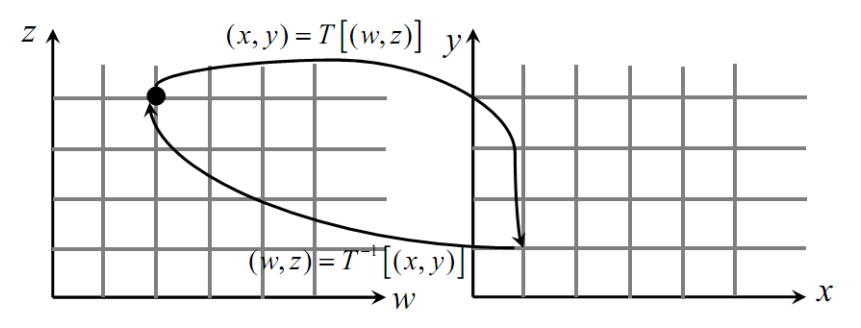
\includegraphics[width = 0.75\linewidth]{fig3.png}
    \caption{Minh họa phép biến đổi T}
    \label{fig3}
\end{figure}

\subsection{Affine transformation}
\begin{figure}[ht!]
    \centering
    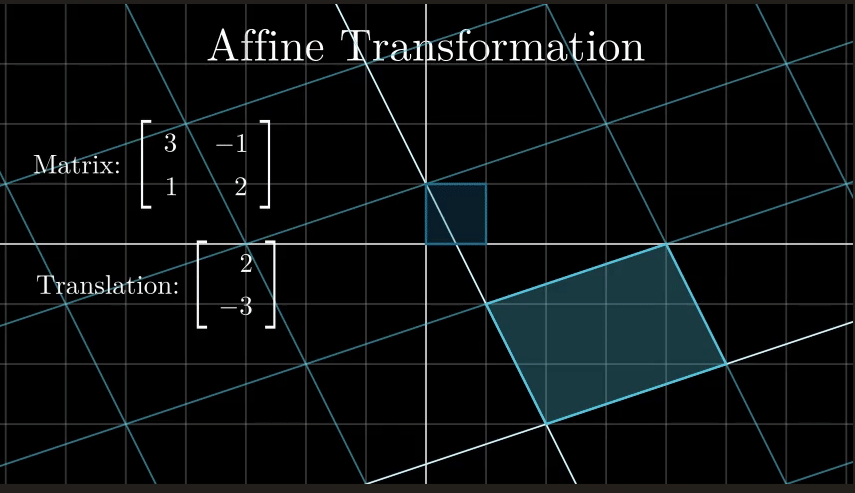
\includegraphics[width = 0.8\linewidth]{fig4.png}
    \caption{Affine Transformation}
    \label{fig4}
\end{figure}
Trong thực tế hiển nhiên không gian $\mathbb{R}^{2}$ là một không gian \textit{affine}. Với hệ tọa độ chuẩn tắc ta có \textit{hệ tọa độ Descartes} quen thuộc. Ý tưởng biến đổi một hình ảnh thành một hình ảnh khác trong cùng mặt phẳng biểu diễn, tương đương với ta tìm một hệ tọa độ khác trong không gian ban đầu!\\
Từ công thức (\ref{eq1}) chính là công thức tổng quát cho đổi các tọa độ trong không gian \textit{affine} nói chung, nhưng cũng là công thức của \textit{phép biến đổi affine}. Tuy nhiên để cho tiện, ta có thể gộp phần $bias$ với tọa độ ban đầu như sau:\\
Đặt $\bar{\textbf{x}'} = [x'; y'; 1]$, $\bar{\textbf{x}} = [x; y; 1]$, và $$\bar{\textbf{A}} = \begin{bmatrix}
a_{11} & a_{12} & t_x\\
a_{21} & a_{22} & t_y\\
0 & 0 & 1
\end{bmatrix} = \begin{bmatrix}
\textbf{A} & \textbf{t}\\
\textbf{0}^{T} & 1
\end{bmatrix}
$$
Ta có phép biến đổi \textit{Affine}:
$$\bar{\textbf{x}'} = \bar{\textbf{A}} \bar{\textbf{x}} $$
Hình \ref{fig4} và hình \ref{fig8} minh họa cho ta về phép biến đổi \textit{affine}.
\begin{figure}[ht!]
    \centering
    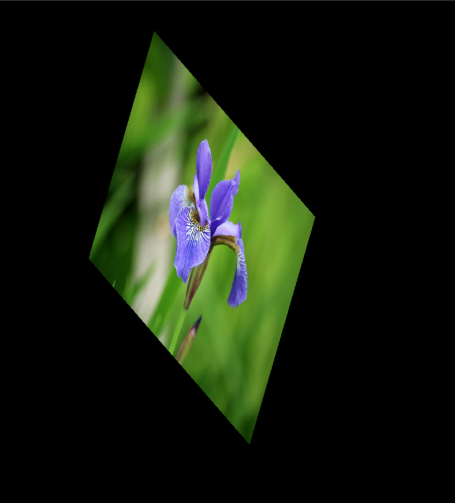
\includegraphics[width = 0.5\linewidth]{fig8.png}
    \caption{Affter using affine transformation}
    \label{fig8}
\end{figure}
\subsection{Projective Transformation}
\subsubsection{Homography}
Hormography là một dạng phép chiếu, cho phép chúng ta tận dụng các phép chiếu để liên hệ giữa hai hình ảnh. Ban đầu, Hormohraphy được giới thiệu để nghiên cứu sự thay đổi giữa các phương diện, và chúng giúp ta có cái nhìn rõ ràng hơn về việc một bức ảnh sẽ thay đổi như thế nào nêu nhìn từ những góc độ khác nhau.\\
Bản chất Hormography là một sự biến đổi giữa hai hình ảnh của cùng một cảnh.\\
Tuy nhiên để có thể làm việc được với Homography, ta phải hiểu đơn giản được về nguyên lí hoạt động của máy ảnh.\\
\begin{figure}[ht!]
    \centering
    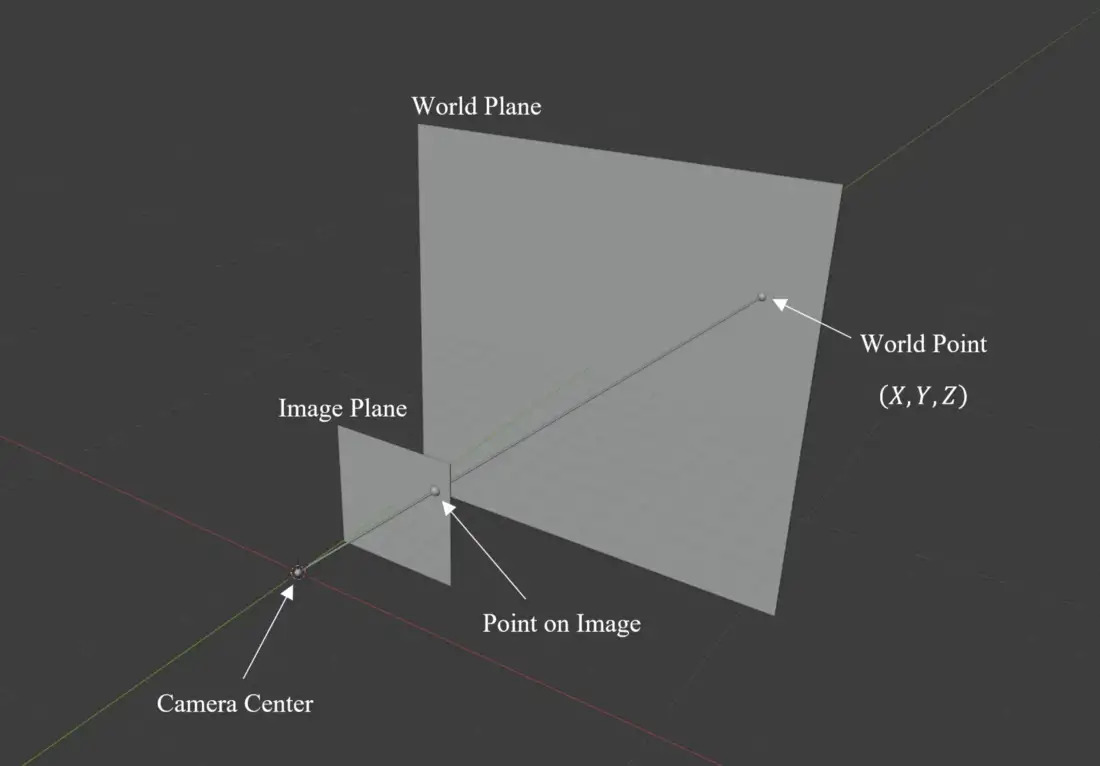
\includegraphics[width = 0.8\linewidth]{fig5.jpg}
    \caption{How camera works.}
    \label{fig5}
\end{figure}
\phantom{a}\\
Như hình \ref{fig5}, ta có thể giả giử thế giới chúng ta đối với camera là một mặt phẳng (\textit{World Plane}) và ảnh sẽ được thu ở trên mặt phẳng ảnh (\textit{Image Plane}). Một điểm thu được trên mặt phẳng ảnh, thu được bằng cách chiếu một tia sáng từ điểm đặt camera xuyên qua điểm đó, giao điểm giữa tia sáng là mặt phẳng ảnh sẽ là điểm ta cần tìm.
\subsubsection{Homography Coordinates}
Hormography Coordinates (Hệ tọa độ đồng nhất) là một hệ tọa độ đặc biệt, bên cạnh hệ tọa độ \textit{Descartes} là chúng ta biết. Hệ tọa độ này được ra đời bởi lí do: Ta không thể biểu diễn được một điểm ở vô hạn trên mặt phẳng \textit{Descartes}.\\
Một điểm trong hệ tọa độ đồng nhất, sẽ yêu cầu 3 thông số (tọa độ) $[x';y';z']$. Để chuyển từ hệ tọa độ đồng nhất sang hệ tọa độ \textit{Descartes} rất đơn giản như sau:
\begin{equation}
    [x';y';z'] \rightarrow [x,y]: \begin{cases}
        x = x'/z'\\y=y'/z'
    \end{cases}
    \label{eq2}
\end{equation}
Nhìn vào (\ref{eq2}), ta có một vài nhận xét thú vị sau:
\begin{enumerate}
    \item Khi $z' \rightarrow 0$, ta có điểm vô cực.
    \item \ldots Xem thêm ở đây: \href{https://towardsdatascience.com/understanding-transformations-in-computer-vision-b001f49a9e61}{Understanding transformations in computer vision - towardsdatascience.com}
\end{enumerate}
\subsubsection*{A different side}
Có lẽ khái niệm trên sẽ không làm hài lòng nhiều người, tôi cũng vậy, tôi sẽ đưa ra một cách nhìn khác về hệ tọa độ đồng nhất, và lí do tại sao ta lại có công thức (\ref{eq2}). \\
\begin{figure}[ht!]
    \centering
    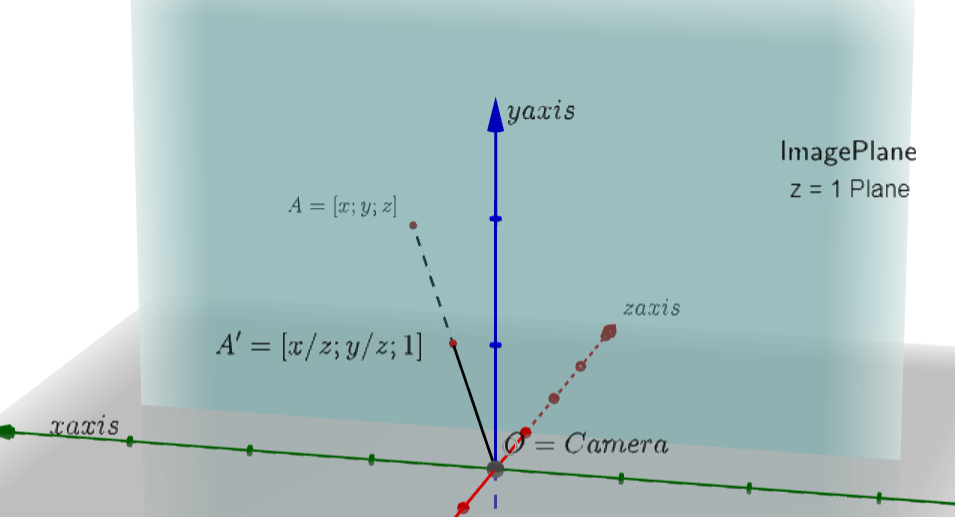
\includegraphics[width = 0.8\linewidth]{fig6.png}
    \caption{A different side}
    \label{fig6}
\end{figure}
Nếu ta quy ước mặt phẳng chiếu của chúng ta là mặt phẳng $z = 1$, và camera được đặt tại gốc tọa độ thì sao? Chỉ đơn giản với \textit{Định lí Thales}, chẳng phải khi đó, điểm mà ta thu được trên mặt phẳng chiếu cũng có dạng tương tự như công thức (\ref{eq2}) hay sao?  (Hình \ref{fig6})\\
Tuy nhiên chúng ta không được đánh đồng điều trên với hệ tọa độ đồng nhất. Nhưng từ giờ tôi sẽ dùng góc nhìn này để suy ra những điều khác. Bởi lẽ, nó sẽ cho ta cảm giác quen thuộc đã đành, nhưng còn bởi ta sẽ sử dụng kết quả mà ta đã thu được từ không gian \textit{affine}. (\textit{Xem lại phần \ref{n1}}).
\subsubsection{Equation of Homography}
Như đã đề cập ở trên, ta cần tìm mối liên hệ giữa hai bức ảnh thu được từ hai góc độ khác nhau, điều này hoàn toàn tương đương với một hệ tọa độ $(O',i',j',k')$ khác trong không gian \textit{affine} $\mathbb{R}^{3}$.\\
Từ công thức (\ref{eq1}), ta có tọa độ mới của một điểm sau khi đổi hệ tọa độ là:
\begin{equation}
\begin{bmatrix}
    x'\\y'\\z'
\end{bmatrix} = \begin{bmatrix}
    C_{11}&C_{12}&C_{13}\\
    C_{21}&C_{22}&C_{23}\\
    C_{31}&C_{32}&C_{33}
\end{bmatrix}\begin{bmatrix}
    x\\y\\z
\end{bmatrix}+\begin{bmatrix}
    t_1\\t_2\\t_3
\end{bmatrix}
\label{eq3}
\end{equation}
Đến đây ta có thể sử dụng \textit{bias trick} như trên. Tuy nhiên như thế kết quả sẽ không đẹp, cho nên công thức (\ref{eq3}) có thể viết lại như sau:
\begin{equation}
\begin{bmatrix}
    x'\\y'\\z'
\end{bmatrix} = \begin{bmatrix}
    C_{11}&C_{12}&C_{13}&C_{14}\\
    C_{21}&C_{22}&C_{23}&C_{24}\\
    C_{31}&C_{32}&C_{33}&C_{34}
\end{bmatrix}\begin{bmatrix}
    x\\y\\z\\1
\end{bmatrix}
\label{eq4}
\end{equation}
\underline{Chú ý}: Các tọa độ trên cùng là tọa độ trong không gian đồng nhất.\\
Do đó, ta có nhận xét rằng, nếu nhân vào cả hai vế của phương trình (\ref{eq4}) một số nào đó, sau cùng khi chuyển về hệ tọa độ \textit{Descartes} số đó vẫn sẽ bị triệt tiêu. Điều này có ý nghĩa lớn, đó là ta có thể giảm tham số cho ma trận \textit{Homography}, tức là giảm số biến cần phải giải. Điều này khá giống với điều ta làm với đường thằng trong hệ tọa độ \textit{Dercates}. Từ $ax+by+c =0$ hoàn toàn tương đương $y = a'x+b'$.\\
Quy ước, thường set vị trí $C_{34} = 1$. Thật vậy, để tổng quát, ta rút $C_{34}$ ra ngoài. Khi đó phương trình (\ref{eq4}) trở thành:
\begin{equation}
\begin{bmatrix}
    x'\\y'\\z'
\end{bmatrix} = \alpha \begin{bmatrix}
    h_{11}&h_{12}&h_{13}&h_{14}\\
    h_{21}&h_{22}&h_{23}&h_{24}\\
    h_{31}&h_{32}&h_{33}&1
\end{bmatrix}\begin{bmatrix}
    x\\y\\z\\1
\end{bmatrix}
\label{eq5}
\end{equation}
\begin{figure}[ht!]
    \centering
    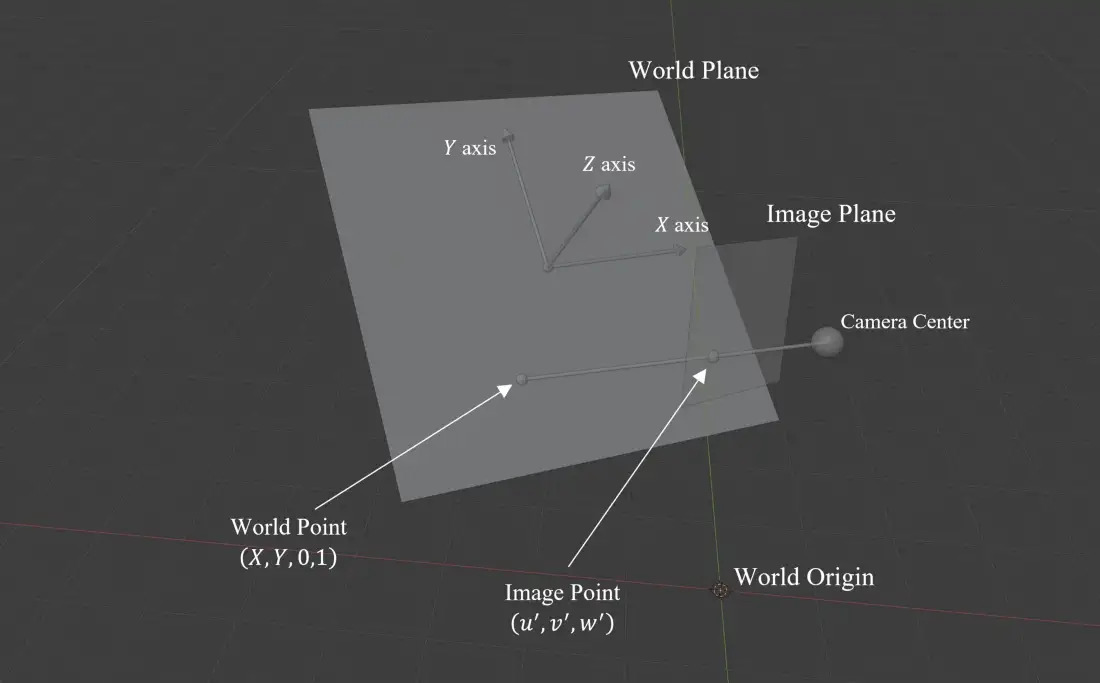
\includegraphics[width = 0.8\linewidth]{fig7.jpg}
    \caption{Convenient choice of coordinate systems}
    \label{fig7}
\end{figure}
Cuối cùng, điều này khá `ảo'. Đó là ta sẽ set vị trí cho mặt phẳng thế giới (\textit{World Plane} - Hình \ref{fig5}). Điều này là vô cùng hợp lí, dù khá vô lí :)). Thật vậy, ta giả sử mặt phẳng thế giới của ta thỏa tất cả các điểm trên đó, cao độ đều bằng 0, tức là mặt phẳng ấy sẽ đi qua gốc tọa độ và vuông góc với \textit{vector} cao độ (Hình \ref{fig7}). Khi đó phương trình (\ref{eq5}) sẽ là:
\begin{equation}
\begin{bmatrix}
    x'\\y'\\z'
\end{bmatrix} = \alpha \begin{bmatrix}
    h_{11}&h_{12}&h_{13}&h_{14}\\
    h_{21}&h_{22}&h_{23}&h_{24}\\
    h_{31}&h_{32}&h_{33}&1
\end{bmatrix}\begin{bmatrix}
    x\\y\\0\\1
\end{bmatrix}
\label{eq6}
\end{equation}
Đến đây, ta có thể bỏ đi cột thứ 3 của \textit{Homography matrix}. Kết quả cuối cùng thu được sẽ là:
\begin{equation}
\begin{bmatrix}
    x'\\y'\\z'
\end{bmatrix} = \alpha \begin{bmatrix}
    h_{11}&h_{12}&h_{14}\\
    h_{21}&h_{22}&h_{24}\\
    h_{31}&h_{32}&1
\end{bmatrix}\begin{bmatrix}
    x\\y\\1
\end{bmatrix}
\label{eq7}
\end{equation}
Viết lại:
\begin{equation}
\begin{bmatrix}
    x'\\y'\\z'
\end{bmatrix} = \alpha \begin{bmatrix}
    h_{11}&h_{12}&h_{13}\\
    h_{21}&h_{22}&h_{23}\\
    h_{31}&h_{32}&1
\end{bmatrix}\begin{bmatrix}
    x\\y\\1
\end{bmatrix}
\label{eq8}
\end{equation}
Ma trận ở thu được ở vế phải được gọi là ma trận đồng nhất (\textit{hormography matrix})
\subsubsection{Starting from the camera structure}
Thật ra điều trên có thể suy ra được từ cấu tạo của máy ảnh. Ma trận trên thu được bằng cách hợp các bộ phận nhỏ của máy ảnh, với từng chức năng cụ thể của chúng. Dưới đây là mô hình máy ảnh lỗ kim (\textit{Pinhole Camera model}) (\textit{là một thiết bị chụp ảnh đơn giản không có ống kính, thay vào đó, một lỗ kim với một khẩu độ nhỏ duy nhất – chính là nơi tiếp nhận hình ảnh – được tạo ra trên một mặt của hộp kín.})
\begin{equation}
\begin{bmatrix}
    x'\\y'\\z'
\end{bmatrix} = \begin{bmatrix}
    f_x&0&c_x&0\\
    0&f_y&c_y&0\\
    0&0&1&0
\end{bmatrix}
\begin{bmatrix}
    r_{11}&r_{12}&r_{13}&t_{1}\\
    r_{21}&r_{22}&r_{23}&t_{2}\\
    r_{31}&r_{32}&r_{33}&t_{3}\\
    0&0&0&1
\end{bmatrix}
\begin{bmatrix}
    x\\y\\z\\1
\end{bmatrix}
\label{eq9}
\end{equation}
Trong đó, ma trận đầu tiên từ phải sang còn được gọi là Camera ngoài - \textit{Camera Extinsic matrix}, nó cung cấp cho chúng ta về vị trí của \textit{camera} trong không gian 3 chiều. Ma trận còn lại được gọi là Camera trong - \textit{Camera Intric} chức năng là biến ảnh thật thành ảnh số. Nhân tung tóe ta sẽ có lại những kết quả trên.

\subsubsection{Calculating the Entries of the Homography Matrix}
Để tìm được ma trận đồng nhất, bẩn nhất ta phải giải một hệ phương trình 8 ẩn (4 cặp đỉnh). Và \ldots đây là ý tưởng người ta thường sử dụng. Ta sẽ xây dựng hệ phương trình như sau:\\
Đầu tiên, từ phương trình (\ref{eq8}) ta suy ra:
\begin{equation}
\begin{bmatrix}
    x'/z'\\y'/z'\\1'
\end{bmatrix} = z'\alpha \begin{bmatrix}
    h_{11}&h_{12}&h_{14}\\
    h_{21}&h_{22}&h_{24}\\
    h_{31}&h_{32}&1
\end{bmatrix}\begin{bmatrix}
    x\\y\\1
\end{bmatrix}
\label{eq10}
\end{equation}
Đặt $u = x'/z'$, $v = y'/z', z'\alpha = \mu$, khi đó ta có tọa độ điểm sau biến đổi trong hệ tọa độ \textit{Descartes} như đã nói ở trên.\\
%\underline{Nhận xét:} Ta biết rằng, ảnh của ta bản chất là tập hợp các điểm ảnh, được đặt trên một hệ tọa độ nguyên dương. Do đó tọa độ điểm ảnh phải nguyên, tức ảnh sau một phép biến đổi hình học bất kì cần được nội suy để đạt được ảnh mới với sai số nhỏ. (Điều này ta sẽ thảo luận sau)\\%
Khi đó từ phương trình (\ref{eq10}), ta có hệ phương trình sau:
\begin{equation}
\begin{cases}
u/\mu = h_{11}.x+h_{12}.y+h_{13}\\
v/\mu = h_{21}.x+h_{22}.y+h_{23}\\
1/\mu = h_{31}.x+h_{32}.y+1

\end{cases}
\label{eq11}
\end{equation}
Rút thế từ phương trình số 3, thay váo hai phương trình trên ta được:
\begin{equation}
\begin{cases}
h_{11}.x+h_{12}.y+h_{13}-h_{31}.ux-h_{32}.uy-u=0\\
h_{21}.x+h_{22}.y+h_{23}-h_{31}.vx-h_{32}.vy-v = 0
\end{cases}
\label{eq12}
\end{equation}
Tương đương:
\begin{equation}
    \begin{bmatrix}
        x & y&1&0&0&0&-ux&-uy\\
        0&0&0&x&y&1&-vx&-vy
    \end{bmatrix} \begin{bmatrix}
        h_{11}\\h_{12}\\h_{13}\\h_{21}\\h_{22}\\h_{23}\\h_{31}\\h_{32}
    \end{bmatrix} = \begin{bmatrix}
        u\\v
    \end{bmatrix}
\label{eq13}
\end{equation}
Vậy, nếu ta biết trước n cặp điểm, ta có hệ phương trình sau:
\begin{equation}
    \begin{bmatrix}
        x^{(1)} & y^{(1)}&1&0&0&0&-u^{(1)}x^{(1)}&-u^{(1)}y^{(1)}\\
        0&0&0&x^{(1)}&y^{(1)}&1&-v^{(1)}x^{(1)}&-v^{(1)}y^{(1)}\\
        \vdots&\vdots&\vdots&\vdots&\vdots&\vdots&\vdots&\vdots\\
                x^{(i)} & y^{(i)}&1&0&0&0&-u^{(i)}x^{(i)}&-u^{(i)}y^{(i)}\\
        0&0&0&x^{(i)}&y^{(i)}&1&-v^{(i)}x^{(i)}&-v^{(i)}y^{(i)}\\
        \vdots&\vdots&\vdots&\vdots&\vdots&\vdots&\vdots&\vdots&\\
                x^{(n)} & y^{(n)}&1&0&0&0&-u^{(n)}x^{(n)}&-u^{(n)}y^{(n)}\\
        0&0&0&x^{(n)}&y^{(n)}&1&-v^{(n)}x^{(n)}&-v^{(n)}y^{(n)}\\
    \end{bmatrix} \begin{bmatrix}
        h_{11}\\h_{12}\\h_{13}\\h_{21}\\h_{22}\\h_{23}\\h_{31}\\h_{32}
    \end{bmatrix} = \begin{bmatrix}
        u^{(1)}\\v^{(1)}\\ \vdots\\u^{(i)}\\v^{(i)}\\ \vdots \\ u^{(n)}\\v^{(n)}
    \end{bmatrix}
    \label{eq14}
\end{equation}
\underline{Nhận xét:} Ở đây số phương trình của ta tối thiểu là 8, tức 4 cặp điểm biết trước. Tuy nhiên ta có thể cung cấp nhiều điểm hơn, càng nhiều thì kết quả càng chính xác. Tất nhiên, hệ phương trình trên, nếu quá số ẩn, dù cho xác định chính xác đi chăng nữa vẫn có khả năng vô nghiệm rất cao (vì thực tế, tọa độ của ít nhất một trong xác điểm ở trên đã được sấp xỉ - vì ảnh số). Nhưng nó lại càng rõ ràng một điều rằng nếu hệ của ta càng nhiều phương trình thì càng chính xác. Câu hỏi đặt ra: Vậy tính như thế nào?\\ 
Bạo dạn đoán đi! Ta thấy mô hình trên khá giống với mô hình hồi quy tuyến tính (\textit{linear regression}) (\textit{ta sẽ bàn luận trong bài tiếp theo}). Ta cùng thử:\\\\
Đặt ma trận to đùng trong phương trình (\ref{eq14}) là \textbf{W}, còn ma trận cột gồm các phần tử của ma trận \textbf{H} ta đặt là \textbf{x}. Vế phải ta đặt là $\textbf{y}$. Khi đó yêu cầu bài toán tương đương: Tìm \textit{vector} \textbf{x} sao cho $$L = ||\textbf{W}\textbf{x}-\textbf{y}||_{2}^{2} $$ đạt giá trị nhỏ nhất.\\
$$\nabla_{\textbf{x}}L = 2\mbox{}\textbf{W}^{T}(\textbf{W}\textbf{x}-\textbf{y})$$
Tương đương:
\begin{equation}
    \textbf{x} = (\textbf{W}^{T}\textbf{W})^{\dagger}\mbox{}\textbf{W}\textbf{y}
\label{eq15}
\end{equation}
Phương trình (\ref{eq15}) cho ta công thức tính các hệ số của ma trận đồng nhất.\\\\
\underline{Tuy nhiên:} Phương pháp này không hiệu quả đâu :)). Thực tế khi làm việc với các phép biến đổi hình học để biến đổi một ảnh, người ta thường dùng các điểm đặc biệt, có tính bất biến, một trong số đó là các góc của vật thể. Mà hiển nhiên các góc của vật thể không tuyến tính. Nên ngoài thực tế người ta sẽ có cách làm khác (\textit{tôi quên mất r :))). Nếu có thời gian tôi sẽ quay lại tiếp phần này!}).\\
\underline{Chú ý:} Để giải được hệ phương trình thỏa mãn những yêu cầu trên, ta sẽ sử dụng hàm \textit{lstlq} (Return the least-squares solution to a linear matrix equation) của thư viện đại số tuyến tính!
\begin{figure}[ht!]
    \centering
    \begin{subfigure}[b]{0.4\linewidth}             
\includegraphics[width=\linewidth]{im2.jpg}
    \caption{Original Image}
    \end{subfigure}
    \begin{subfigure}[b]{0.38\linewidth}           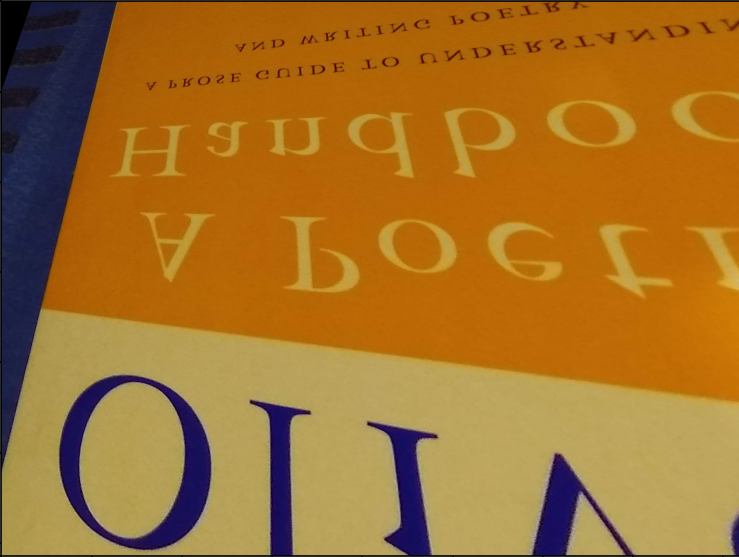
\includegraphics[width=\linewidth]{171_3.png}
    \caption{Àfter that}
    \end{subfigure}

    \begin{subfigure}[b]{0.38\linewidth}           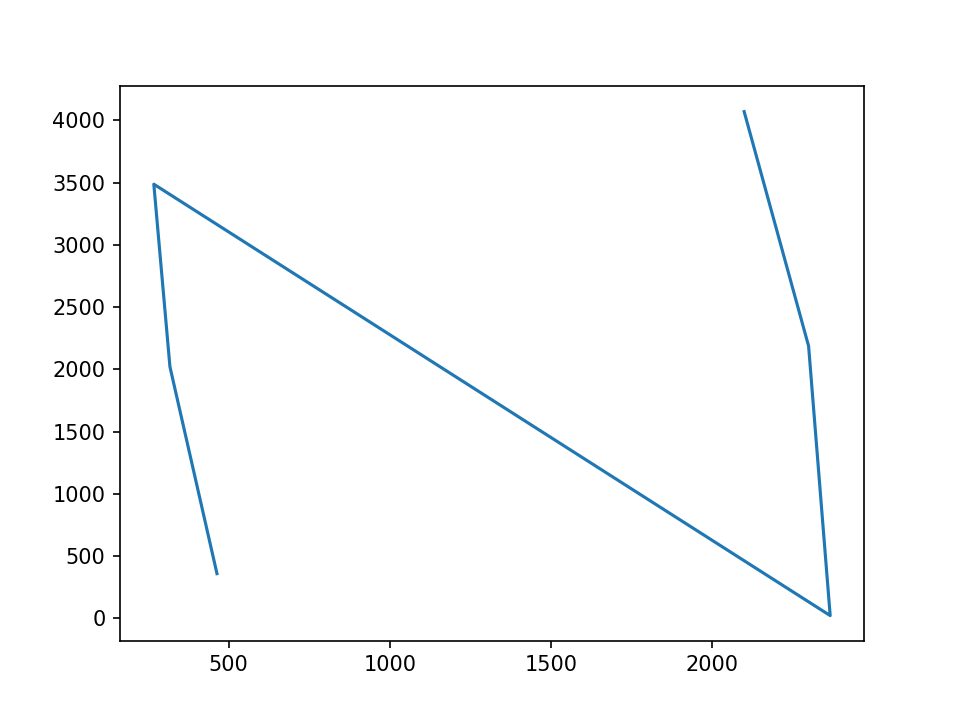
\includegraphics[width=\linewidth]{171_2.png}
    \caption{Source points}
    \end{subfigure}
    \caption{Using Linear Regression Optimization}
    \label{im21}
\end{figure}
\phantom{a}\\
Hình \ref{fig9} minh họa cho ta kết quả của phép biến đổi \textit{projective}
\begin{figure}[ht!]
    \centering
    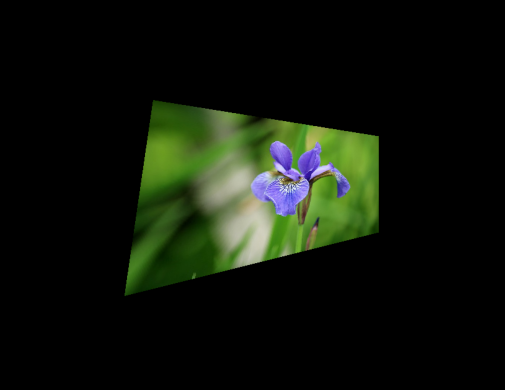
\includegraphics[width = 0.6\linewidth]{fig9.png}
    \caption{After using projective transformation}
    \label{fig9}
\end{figure}
\subsection{Áp dụng phép biến đổi hình học cho ảnh}
Nói lí thuyết thì dễ, nhưng thực tế để áp dụng các phép biến đổi trên biến ảnh cũ thành ảnh mới thì nó không dễ như vậy! Bởi như tôi đã nói, ảnh của ta là bản chất là tập hợp của các điểm ảnh có giá trị, được đặt tại các điểm $(x,y)$ nguyên trong mặt phẳng \textit{Descartes} với gốc tọa độ ở trên góc, trục x hướng xuống, và trục y hướng sang phải. Điều này có nghĩa là cứ cho một điểm ảnh gốc có các tọa độ nguyên, thì điều đấy không có nghĩa rằng điểm mới của điểm đó cũng có tọa độ nguyên! Cho nên ta cần phải `xấp xỉ' ảnh từ lí thuyết thành một ảnh có thể biểu diễn được! Công việc đó được gọi là \textit{Nội suy} (ta sẽ đề cập trong phần sau: phần \ref{n3}).\\
Đến đây, để nội suy ta có hai hướng:
\begin{enumerate}
    \item Chiếu tọa độ ảnh gốc lên tọa độ ảnh mới và xấp xỉ (\textit{chiếu thuận})
    \item Ngược lại (\textit{chiếu đảo})
\end{enumerate}
\begin{figure}[ht!]
    \centering
    \begin{subfigure}[b]{0.8\linewidth}
        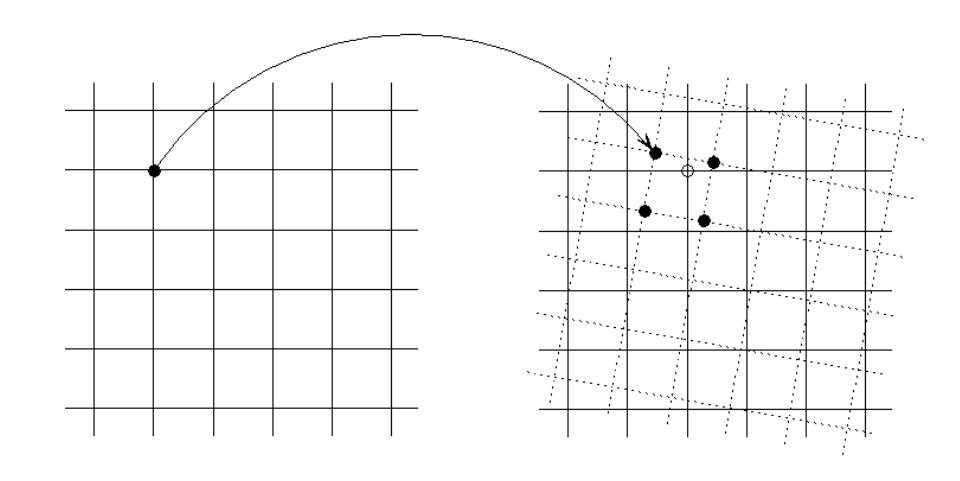
\includegraphics[width = \linewidth]{fig11a.png}
        \caption{Chiếu thuận}
    \end{subfigure}
    \begin{subfigure}[b]{0.8\linewidth}
        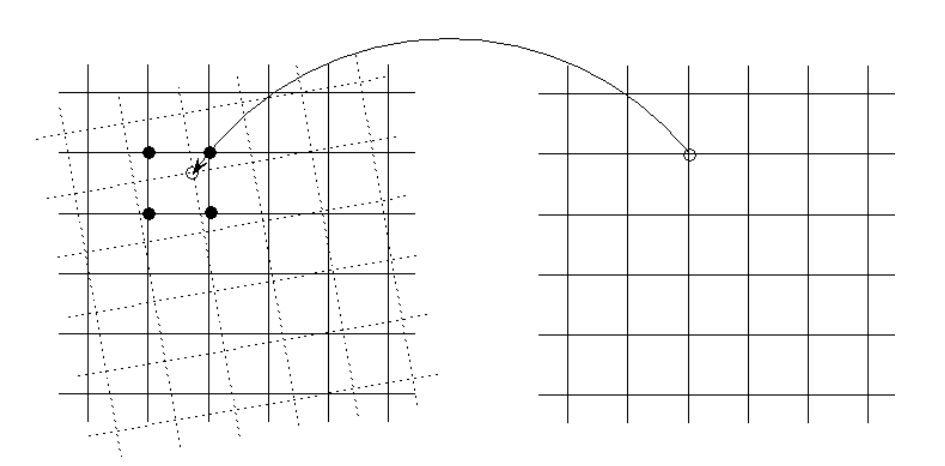
\includegraphics[width = \linewidth]{fig11b.png}
        \caption{Chiếu đảo}
    \end{subfigure}
    \caption{Hai hướng xấp xỉ}
    \label{fig11}
\end{figure}
Ta thấy, nếu sử dụng cách thứ nhất giả sử như ta theo phương pháp NN (\ref{n3}) đi, thì có thể bị trường hợp 2 \textit{pixel} ảnh gốc cùng chui vào một \textit{pixel} ảnh mới. Còn nếu sử dụng BILINEAR (\ref{n3}) thì có thể có nhiều hơn một điểm ảnh của ảnh mới trong bộ bốn điểm ảnh của ảnh cũ. Trong khi nếu dùng cách thứ hai thì hoàn toàn không xảy ra những điều trên, lại có thể tận dụng các kết quả về nội suy trước đó để tính toán!\\
Vậy để làm theo cách thứ hai, cụ thể có các bước sau:
\begin{enumerate}
    \item Set trước một `khung ảnh', tính ảnh tọa độ ảnh cũ $(x, y)$ của tọa độ ảnh mới $(x', y')$ của khung ảnh trên. $(x,y) = T^{-1}(x',y')$
    \item Nội suy (phần \ref{n3})
\end{enumerate}
Bước đầu, khá đơn giản, nói bằng lời chắc cũng đã hiểu. Còn bước thứ hai, ta sẽ đi sâu hơn trong phần sau đây!
\subsection{Interpolation}
\label{n3}
Đây là phần nội dung chính cuối cùng mà tôi muốn đề cập. Nội suy (\textit{Interpolation}), thuật ngữ này nếu còn mới lạ thì chỉ cần hiểu đơn giản: Nội suy là phương pháp ước tính giá trị của các điểm dữ liệu chưa biết trong phạm vi của một tập hợp rời rạc chứa một số điểm dữ liệu đã biết. (\href{https://vi.wikipedia.org/wiki/N%E1%BB%99i_suy}{Nội suy - Wikipedia}).\\
Một số phương pháp nội suy đã và đang được sử dụng rất nhiều trong các thư viện xử lí ảnh của các ngôn ngữ lập trình nổi tiếng, nhưng phổ biến nhất là 3 phương pháp nội suy sau: NN (\textit{Nearest Neighbor}), BILINEAR và BICUBIC, chẳng hạn như trong Matlab hay trong thư viện OpenCV của Python, \ldots\\
Trong 3 phép nội suy phổ biến trên, tôi sẽ chỉ giới thiệu hai phương pháp là: NN và BILINEAR, bởi BICUBIC một phần vì phức tạp, nhưng bản chất cũng giống BILINEAR chỉ khác là thay vì sử dụng 4 lân cận, nó dùng 16 lân cận.

\subsubsection{NN}
\subsubsection*{Tổng quát:} Ta có tập hợp $\textbf{A} = \{a_1, a_2, \ldots, a_n\}$ có giá trị $f(\textbf{A}) = \{f_1, f_2, \ldots, f_n\}$. Khi đó giá trị của điểm $A$ chưa biết sẽ bằng giá trị của điểm gần nó nhất trong \textbf{A}. Khoảng cách đây có thể là một \textit{metric} bất kì.
\begin{figure}[ht!]
\centering
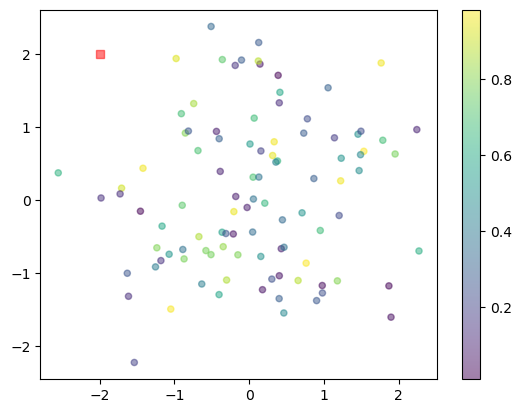
\includegraphics[width = 0.8\linewidth]{fig10.png}
\caption{Nearest Neighbor}
\label{fig10}
\end{figure}
\phantom{a}\\
Giả sử trong hình \ref{fig10}, các điểm biết giá trị của ta là các điểm hình tròn trong không gian hai chiều, giá trị của chúng được thể hiện bằng màu sắc. Còn điểm màu đỏ là điểm mà ta cần phải đi xấp xỉ giá trị của nó.\\
Dễ thấy điểm gần nhất điểm đó là điểm màu vàng, cho ta giá trị ước tính của điểm màu đỏ là khoảng 0.9.
\subsubsection*{Trong các phép biến đổi hình học:}
Tiếp tục bước hai dang dở ở trên, sau khi tính được tọa độ $(x,y) = T^{-1}(x',y')$ gọi $(\hat{x}, \hat{y})$ là tọa độ điểm ảnh xấp xỉ của $(x, y)$. Vơi NN, $(\hat{x},\hat{y}) = \text{round}(x,y)$. Khi đó giá trị điểm ảnh $(x',y')$ của ảnh mới sẽ được gán bằng giá trị của $(\hat{x}, \hat{y})$ trong ảnh cũ!

\subsubsection{BILINEAR}
BILINEAR - nội suy song tuyến tính. Trước tiên để hiểu khái niệm này ta cần phải hiểu sơ lược về nội suy tuyến tính.
\subsubsection*{Nội suy tuyến tính}
\textbf{Bài toán:} Cho hai điểm $A(a,f(a))$, $B(b, f(b)$, $C(c,?)$ là điểm nằm giữa $A$ và $B$. Hãy ước tính $f(c)$ bằng phương pháp nội suy tuyến tính.\\
\underline{Giải}\\
Nội suy tuyến tính, tức ta dự đoán mô hình sẽ có dạng tuyến tính. Với giả thiết này ta suy ra, nếu biết phương trình đường thằng đi qua $A$ và $B$ ta sẽ xác định được giá trị tại $c$. Thật vậy, ta có phương trình tổng quát đường thẳng $\Delta$ đi qua $A, B$:
$$y = \frac{f(b)-f(a)}{b-a}(x-a)+f(a)$$
suy ra \begin{equation}
    f(c) = y(c) = f(a)\frac{b-c}{b-a}+f(b)\frac{c-a}{b-a}
    \label{eq16}
\end{equation}
\underline{Nhận xét:} Nếu ta đặt $t = \frac{b-c}{b-a}$, ta còn có công thức đẹp hơn, tổng quát hơn: $f(c) = tf(a)+(1-t)f(b), \text{with }t \in [0,1]$. Đây chính là định lí giá trị trung bình tôi đã đề cập trong bài trước. Ngoài ra, nó còn chính là khởi nguồn cho định nghĩa về \textit{hàm lồi}!\\
Nhận xét thế thôi, nhưng ta sẽ sử dụng trực tiếp công thức (\ref{eq16}) trong bài này!
\subsubsection*{Nội suy song tuyến tính}
\begin{figure}[ht!]
    \centering
    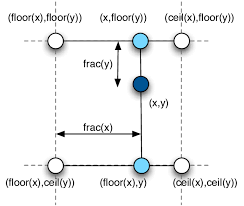
\includegraphics[width = 0.4\linewidth]{fig12.png}
    \caption{BILINEAR Interpolation}
    \label{fig12}
\end{figure}
\phantom{a}\\
Như hình \ref{fig12}, ta có 4 lân cận màu trắng của điểm màu xanh đậm tạo thành hình chữ nhật. Khi đó để ước tính giá trị của điểm màu xanh đậm ta làm như sau: Đầu tiên sử dụng hồi quy tuyến tính cho hai điểm bên trên ta được điểm mới đầu tiên (màu xanh nhạt). Tương tự với hai điểm phía dưới ta được điểm mới thứ hai (cũng màu xanh nhạt). Cuối cùng ta áp dụng hồi quy tuyến tính cho hai điểm vừa mới tìm được!\\
Cách làm ở bước 2 trong trường hợp này, y hệt mô tả trên!
\begin{figure}[ht!]
    \centering
    \begin{subfigure}[b]{0.7\linewidth}
        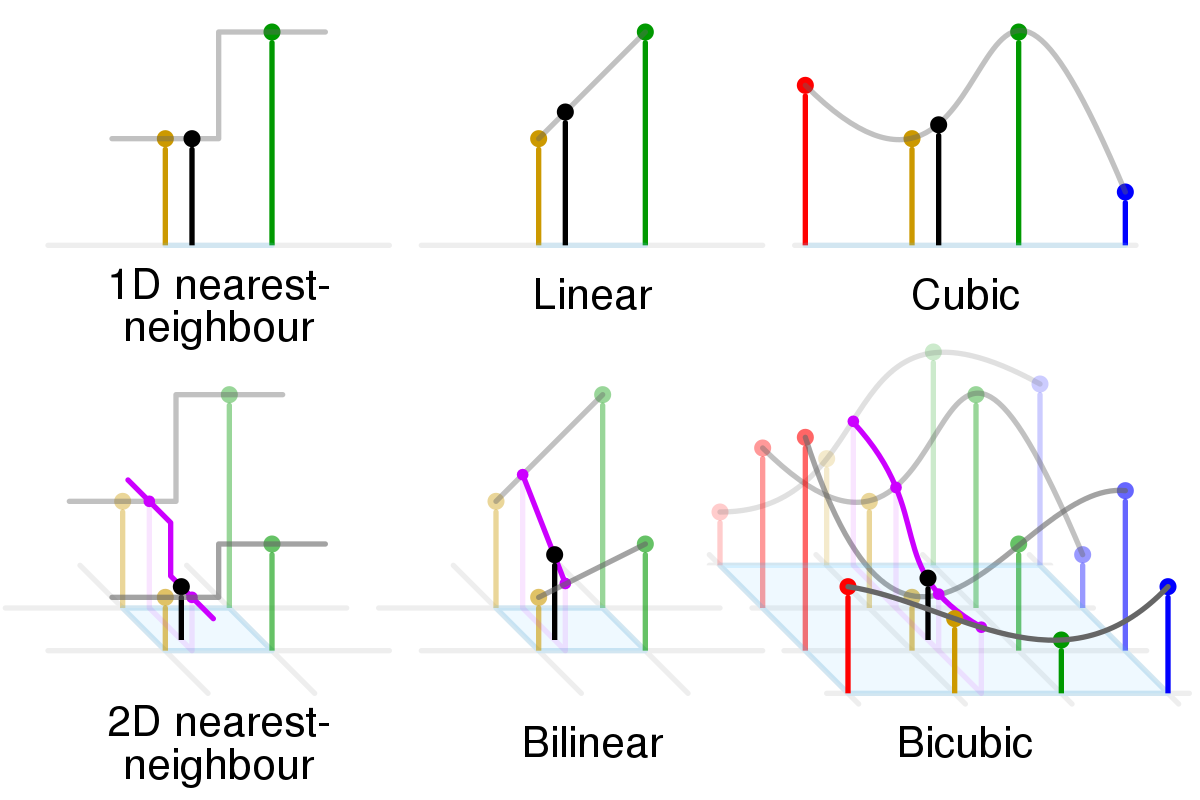
\includegraphics[width = \linewidth]{fig13.png}
        \caption{Interpolation models}
    \end{subfigure}
    \begin{subfigure}[b]{0.8\linewidth}
        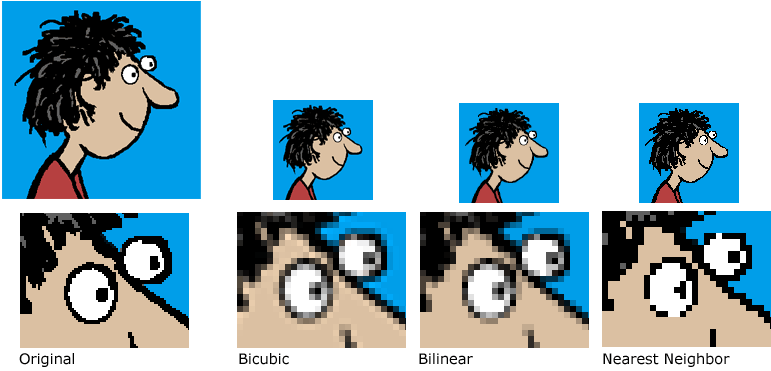
\includegraphics[width = \linewidth]{fig14.png}
        \caption{Results}
    \end{subfigure}
    \caption{Interpolation}
    \label{fig13.5}
\end{figure} \phantom{a}\\\\
Nhìn vào hình \ref{fig13.5} (b), ta thấy rõ được độ hiệu quả đối với từng phép nội suy trên, trong đó BILINEAR và BICUBIC tốt hơn hẳn NN, nhưng BILINEAR và BICUBIC cũng chả khác nhau là bao!\\
Còn về BICUBIC, các bạn có thể mường tượng được trong hình \ref{fig13.5} (a). Tìm hiểu thêm tại \href{https://en.wikipedia.org/wiki/Bicubic_interpolation}{Bicubic interpolation - Wikipedia}.

\subsection{Ứng dụng}
"""
\underline{PS:} Tạm thời phần này tôi xin phép chưa được hoàn thành vì bản thân cũng chưa hoàn thành phần này, thứ hai là tôi cũng đã dành quá nhiều thời gian vào mảng này trong những ngày qua. Đây thực sự là một phần thú vị với tôi! Và tôi cũng có kha khá ý tưởng ở đây! Tôi cũng không phải là không hoàn thành được, nhưng nếu lúc này vứt đi liêm sỉ lấy kết quả của người khác mà không hiểu gì cũng không hay lắm!!! Tôi hi vọng sau khi đi xong một vòng, tôi sẽ quay lại đây, và chúng ta sẽ cùng làm nên những điều tuyệt vời!!!. Hẹn gặp lại vào thời gian gần nhất! 
\\ Nếu bạn cần tự nghiên cứu và tìm hiểu thì có thể tham khảo các trích dẫn dưới đây của tôi! Nó sẽ dẫn đến điều bạn cần!\\
Bài tới chúng ta sẽ bắt đầu nhảy sang ML và DL!\\ """\\
Phép biến đổi hình học như tôi đã giới thiệu vẫn là một hướng thú vị, hay ho và đặc biệt đã có nhiều ứng dụng. Nhưng ở đây tôi chỉ giới thiệu hai ứng dụng cơ bản của nó: \textit{image registration} và \textit{image stitching}.
\subsubsection{Image registration}
\textit{Image registration} dịch sang tiếng việt khá không hay nên tôi sẽ không dùng tiếng việt. \textit{Image registration} hiểu nôm na là đưa các ảnh về cùng một hệ tọa độ. 
\section{Mã nguồn}
Mã nguồn cho bài này có thể tìm thấy tại đây: \href{https://github.com/thuantn210823/Computer-Vision-IPSAL-LAB-}{My Github}.

\newpage
\section{Tài liệu tham khảo}
        \begin{thebibliography}{9}
        \bibitem{slide}
    Truong. PV, Thao. TT \emph{Silde bài giảng tuần 6}, Đại học Bách Khoa Hà Nội.
        \bibitem{slide}
        Harvey Rhody \emph{Lecture 2: Geometric Image Transformations
}, Chester F. Carlson Center for Imaging Science
Rochester Institute of Technology - 2005.
        \bibitem{book}
        Trung. NV \emph{Giáo trình đại số tuyến tính}, Nhà xuất bản Đại học Cuốc gia Hà Nội - 2002.
        \bibitem{book}
        Anh. KQ, Kiet. NA, Man. T, Tuan. ND \emph{Bài tập Đại số tuyến tính và Hình học giải tích}, Nhà xuất bản Đại học Quốc gia Hà Nội - 2002.
    \bibitem{website}
    \href{https://towardsdatascience.com/understanding-homography-a-k-a-perspective-transformation-cacaed5ca17}{Understanding Homography Perspective Tansformation - towardsdatascience.com}
    \bibitem{website}
    \href{https://towardsdatascience.com/understanding-transformations-in-computer-vision-b001f49a9e61}{Understanding Transformations in Computer Vision - towardsdatascience.com}
    \bibitem{website}
    \href{https://towardsdatascience.com/image-panorama-stitching-with-opencv-2402bde6b46c}{Image Panoramo Stitching with OpenCV - towardsdatascience.com}
    \bibitem{website}
    \href{https://en.wikipedia.org/wiki/Bicubic_interpolation}{Bicubic interpolation}
    \bibitem{website}
    \url{https://watkins.cs.queensu.ca/~jstewart/457/notes/06/06-median-bilinear.html}
    \bibitem{website}
    \href{https://vi.wikipedia.org/wiki/N%E1%BB%99i_suy}{Nội suy}
    \end{thebibliography}


\end{document}
